%!TEX root = spadini_davide.tex

\chapter{WebRTC}
\label{cha:webrtc}

WebRTC~\cite{webrtc} is an Application Programming Interface (API) definition drafted by the World Wide Web Consortium (W3C) that supports browser-to-browser applications for voice calling, video chat, and Peer-To-Peer (P2P) file sharing without plugins. It is already implemented in the Chrome, Firefox and Opera browsers. The purpose of WebRTC is to enable rich, high-quality RTC applications to be developed for the browser, mobile platforms, and IoT devices, and allow them all to communicate via a common set of protocols. 

From the point of view of an end-user, WebRTC provides a much simpler way to have real-time conversations with other end-users. It is based on the web technology, thus accessible to any personal or enterprise computer. Without any installation and plugins, users may have exactly the same service which previous stand-alone desktop client provides. WebRTC makes these capabilities accessible to web developers via standard HTML5 tags and JavaScript APIs. For example, we can consider functionality similar to that offered by Skype\footnote{Skype is a free voice-over-IP service and instant messaging client, currently developed by the Microsoft Skype Division.}, but without installing any software or plugin. 

The codecs and protocols used by WebRTC do a huge amount of work to make real-time communication possible, even over unreliable networks (e.g. packet loss concealment, echo cancellation, bandwidth adaptivity, image cleaning, ...)~\cite{started_with_webrtc}. However, WebRTC API still requires a lot of work in order to successfully create the connection between two peers. A fully explation of this process is covered in the Section~\ref{sec:webrtc_signaling}. However, in this project we use the EasyRTC~\cite{easyrtc} framework in order to simplify the creation of the network and its maintenance. More details about this in Section~\ref{sec:easy_tc}.

\section{WebRTC APIs}
\label{sec:webrtc_api}
The main tasks of WebRTC are:
\begin{itemize}
	\item Acquiring audio and video: getting access to the microphone or camera, getting a streaming of media for either of them
	\item Communicating audio and video: being able to connect to another WebRTC end-point through Internet, and send audio and video stream in real-time
	\item Communicating generic data: not only audio and video, but for any arbitrary application data
\end{itemize}
These three main categories are translated in three Javascript APIs:
\begin{itemize}
	\item\textbf{\textsf{MediaStream} (aka getUserMedia)}.
This API is not relevant for this project; in fact, the messages that the peers will exchange are not streams of audio and video, but simple JSON.
	\item\textbf{\RTCPeerConnection}.
This module enables peer-to-peer exchange of arbitrary data, with low latency and high throughput. This is what we use to send data between peers, but still they need to be connected in order to send and receive messages, so the DataChannel is built on top of a \textit{PeerConnection}.
	\item\textbf{\RTCDataChannel}.
This is the WebRTC component that handles stable and efficient communication of streaming data between peers. Figure~\ref{fig:webrtcArchitecture} shows the WebRTC architecture diagram and the role of \RTCPeerConnection: the main thing to understand from this diagram is that \RTCPeerConnection shields web developers from the myriad complexities that lurk beneath. As explained before, we did not use WebRTC for audio and video streaming (the first two columns of the diagram); instead, the next sections focus on how to establish a connection using \RTCPeerConnection.
\end{itemize}

\begin{figure}[ht]
  \centering
  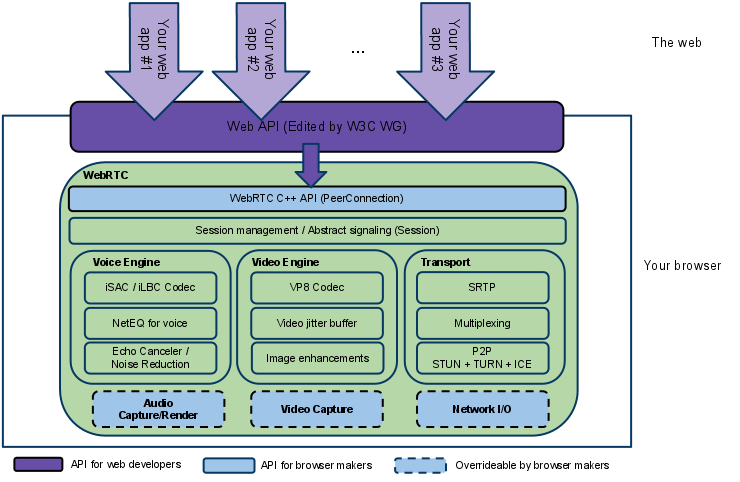
\includegraphics[keepaspectratio=true, width=\textwidth]{images/webrtcArchitecture}\caption{WebRTC architecture (from \url{webrtc.org})}
  \label{fig:webrtcArchitecture}
\end{figure}

\section{WebRTC: Signaling}
\label{sec:webrtc_signaling}
WebRTC uses \RTCPeerConnection to create a connection between peers and communicate audio and video. In order to establish the connection between them it needs a mechanism to coordinate the communication and to send control messages, a process known as signaling. 

Signaling is used to initialize the connection and exchange three types of information:
\begin{itemize}
	\item\textbf{Session control messages}: to initialize or close communication and report errors.
	\item\textbf{Network configuration}: to the outside world, what is my computer's IP address and port?
	\item\textbf{Media capabilities}: what codecs and resolutions can be handled by my browser and the browser it wants to communicate with?
\end{itemize}
The exchange of information via signaling must have successfully completed before peer-to-peer streaming can begin.

Signaling methods and protocols are not specified by WebRTC: signaling is not part of the \RTCPeerConnection API. The web developer can choose the messaging protocol he/she prefer; in this project, WebSockets have been adopted. The reason why the WebRTC group has made this decision is to avoid redundancy and to maximize compatibility with established technologies~\cite{jsep}.

Let us see an example of how to use \RTCPeerConnection: imagine Alice wants to communicate with Bob. To initialize this process, \RTCPeerConnection has two tasks:
\begin{itemize}
	\item Ascertain local media conditions, such as resolution and codec capabilities.
	\item Get potential network addresses for the application's host, known as candidates. (see Section~\ref{sec:webrtc_ice})
\end{itemize}

For the first point, the exchange of media configuration information proceeds using an offer/answer mechanism that is called \JSEP, JavaScript Session Establishment Protocol~\cite{jsep}. Figure~\ref{fig:jsep} shows the \JSEP architecture: both the caller and callee have to save their local session description taken from the browser and send them through some signaling mechanism, then when they receive the session description of the other they set it as the remote session description. Once the process is finished, they both know the configuration of the peer they want to communicate with.

The entire sequence of steps is the following:
\begin{itemize}
	\item Alice creates an \RTCPeerConnection object.
	\item Alice creates an offer using the \RTCPeerConnection \createOffer method.
	\item Alice sets her local description to her offer.
	\item Alice uses a signaling mechanism to send her offer to Bob.
	\item Bob sets his remote description to Alice's offer, so that his \RTCPeerConnection knows about Alice's setup.
	\item Bob create an answer using the \createAnswer function.
	\item Bob sets his answer as the local description.
	\item Bob then uses the signaling mechanism to send his answer back to Alice.
	\item Alice sets Bob's answer as the remote session description.
\end{itemize}
Offers and answers are communicated in Session Description Protocol format (SDP)~\cite{sdp}, which look like this:
\begin{Verbatim}[frame=single]
v=0
o=- 7614219274584779017 2 IN IP4 127.0.0.1
s=-
t=0 0
a=group:BUNDLE audio video
a=msid-semantic: WMS
m=audio 1 RTP/SAVPF 111 103 104 0 8 107 106 105 13 126
c=IN IP4 0.0.0.0
a=rtcp:1 IN IP4 0.0.0.0
a=ice-ufrag:W2TGCZw2NZHuwlnf
a=ice-pwd:xdQEccP40E+P0L5qTyzDgfmW
a=extmap:1 urn:ietf:params:rtp-hdrext:ssrc-audio-level
a=mid:audio
a=rtcp-mux
a=crypto:1 AES_CM_128_HMAC_SHA1_80 inline:9c1AHz27dZ9xPI91YNfSlI67/EMkjHHIHORiClQe
a=rtpmap:111 opus/48000/2
....
\end{Verbatim}
Using this format, the offer and answer messages contain all the necessary information to guarantee that the peers can communicate using the same codecs, resolution and other media capabilities. 
Once this process is finished, and they both know the configuration of the other, they use the ICE Framework in order to establish the connection.

\begin{figure}[ht]
  \centering
  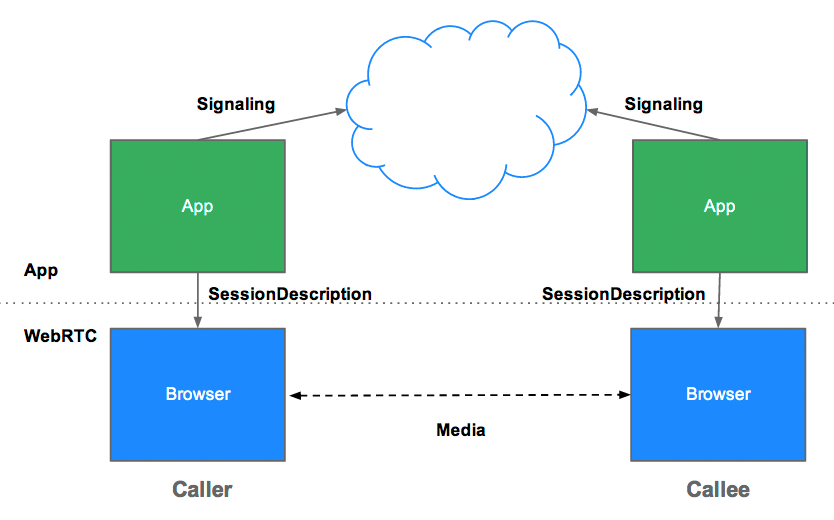
\includegraphics[keepaspectratio=true, width=\textwidth]{images/jsep}\caption{Signaling Diagram}
  \label{fig:jsep}
\end{figure}

\section{WebRTC: ICE Framework}
\label{sec:webrtc_ice}
For metadata signaling, WebRTC applications use an intermediary server, the signaling server, but for actual media and data streaming once a session is established, \RTCPeerConnection attempts to connect clients directly: peer-to-peer. 

In a perfect world, all the nodes are public and they are always reachable. In reality, this is not the case: in fact most devices are behind one or more layers of Network Address Translation (NAT)~\cite{nat}, some have anti-virus software that blocks certain ports and protocols, and many are behind proxies and corporate firewalls. All these configurations make the connection peer-to-peer impossible. However, WebRTC applications can use the Interactive Connectivity Establishment (ICE) framework to overcome the complexities of real-world networking. 

ICE tries to find the best path to connect peers. It tries all possibilities in parallel and chooses the most efficient option that works. ICE first tries to make a connection using the host address obtained from a device's operating system and network card; if that fails (which it will for devices behind NATs) ICE obtains an external address using a Session Traversal Utilities for NAT (\STUN) server, and if that fails, traffic is routed via a Traversal Using Relays around NAT (\TURN) server~\cite{webrtc_infrastructure}. 

In other words, if the direct link fails (that is if the peers are behind a NAT), ICE uses the \STUN server. Figure~\ref{fig:stun} shows how it works: the server has one simple task, find the public IP address and port of the peer and send that address back as a response.  This process enables a WebRTC peer to get a publicly accessible address for itself, and then pass that to the other peer via a signaling mechanism, in order to set up a direct link.

If that fails, \TURN servers can be used as a fallback. These servers have a conceptually simple task, to relay a stream, but unlike \STUN servers, they inherently consume a lot of bandwidth. This is in fact the last chance of the ICE Framework.

Figure~\ref{fig:turn} represents the complete schema.

\begin{figure}[ht]
  \centering
  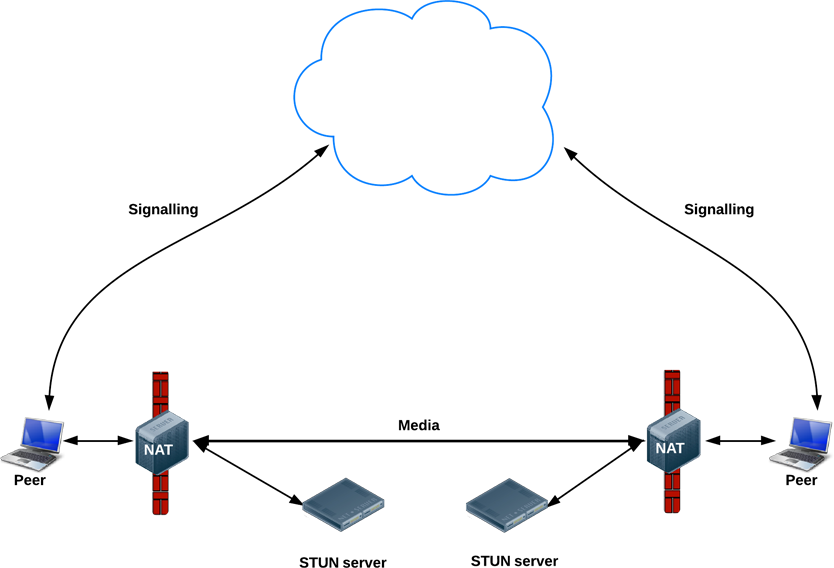
\includegraphics[keepaspectratio=true, width=\textwidth]{images/stun}\caption{Using \STUN servers to get public IP:port addresses}
  \label{fig:stun}
\end{figure}

\begin{figure}[ht]
  \centering
  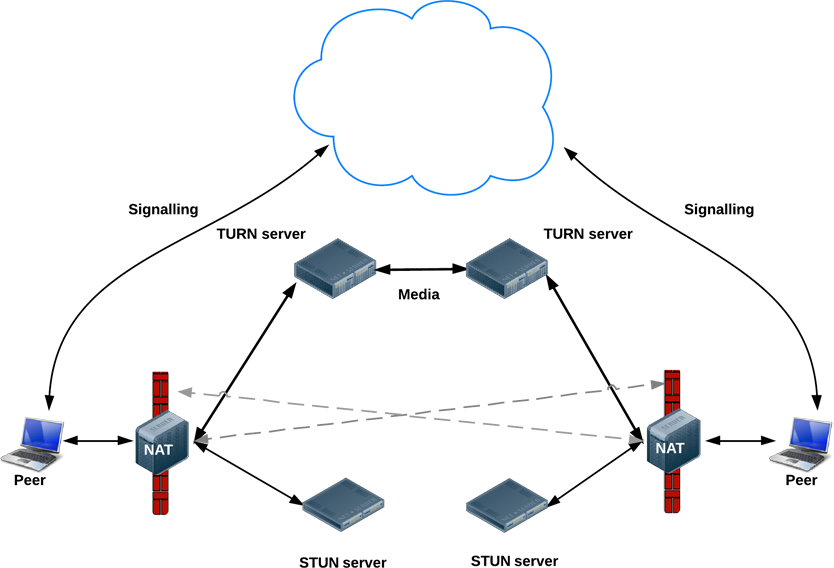
\includegraphics[keepaspectratio=true, width=\textwidth]{images/turn}\caption{The full schema: \STUN, \TURN and signaling}
  \label{fig:turn}
\end{figure}

The URLs of the \STUN and/or \TURN servers are (optionally) specified by the WebRTC application in the configuration object that is the first argument of the \RTCPeerConnection constructor. Once \RTCPeerConnection has these information, it uses the ICE framework to work out the best path between peers, working with \STUN and \TURN servers as necessary. When it find the best solution, it initialize the connection and the peers can start to communicate.

\section{Back to reality: EasyRTC Framework}
\label{sec:easy_tc}
As shown in the previous sections, establishing a connection between two peers in WebRTC is not so simple.
As is often the case with software, with power comes complexity. WebRTC has a learning curve that is likely to hamper its use by web developers. To hide that complexity, Priologic\footnote{A team of Canadian software developers. More information: \url{https://www.priologic.com}} has built the EasyRTC framework.

One of the most important feature of this framework is that, while the WebRTC API requires the developers to implement an involved message passing scheme between clients to establish the peer-to-peer connection, it already provides this schema~\cite{easyrtc} and it is completely hidden from the point of view of the web developers. It is really well documented and there already exists the EasyRTC server (the signaling server) that the nodes will contact in order to register themselves in the network.

EasyRTC is implemented in \textbf{Node.js} and it is available for free.

\subsection{EasyRTC Server}
\label{subsec:easyrtc_server}

The main purpose of the server is to serve the requests of ``join the network'' from the nodes, so it is always listening on a specific port and all the nodes have to be able to reach it. Once a node is registered in the network, has an unique identifier that will be valid until it will disconnect. This ID will identify the node within the network, so the other nodes will have to use it in order to contact that specific peer. 

When a node wants to connect to another one, the request pass through this server that will take care of creating the connection between them. Once the connection has been created, the nodes can communicate without passing through the server. 

As explained before, the signaling mechanism is not part of the WebRTC: EasyRTC server by default uses WebSockets\footnote{EasyRTC server by default uses the \emph{socket.io} module. More information: \url{http://socket.io}}. One advantage of this technique is that through the heartbeats (already implemented inside WebSockets) the server knows which nodes are on-line and which ones have disconnected or crashed. In fact every $N$ seconds (by default $N = 25$ seconds), the server sends an heartbeat to the node and if the node does not reply within the heartbeat timeout (by default it is 60 seconds) it closes the connection with it. We use this technique to capture the failure of a node (it could be crashed or simply disconnected) and send to all the other nodes an advice. If a node was connected to the failed node, it has to replace the broken link with a new one and to do so it contacts the tracker (more information in Section~\ref{cha:tracker}).

\section{SPOF}
A final issue to be considered is related to the ``Single Point Of Failure'' (SPOF): in our system, if the EasyRTC server crashes or for some reason it is no more reachable from the outside world, no-one can join the network and, especially, no-one can capture the failure of another node (in fact this event is triggered only by the server). Handling this situation is not part of my project, since we start from the assumption that the server is always on-line.

However, there is the possibility to add redundancy in the system, creating more than one server in order to have some of them that acts as backup servers. Then, each node decides which of them to contact, and if for some reasons that server goes down, it connects to another one. In this way the problem is solved, but as explained before this was not the task of the project, so for simplicity we implement only one server and we assume that is always reachable.
